% Copyright © 2013 Martin Ueding <dev@martin-ueding.de>

% Copyright © 2012-2013 Martin Ueding <dev@martin-ueding.de>

% This is my general purpose LaTeX header file for writing German documents.
% Ideally, you include this using a simple ``% Copyright © 2012-2013 Martin Ueding <dev@martin-ueding.de>

% This is my general purpose LaTeX header file for writing German documents.
% Ideally, you include this using a simple ``% Copyright © 2012-2013 Martin Ueding <dev@martin-ueding.de>

% This is my general purpose LaTeX header file for writing German documents.
% Ideally, you include this using a simple ``\input{header.tex}`` in your main
% document and start with ``\title`` and ``\begin{document}`` afterwards.

% If you need to add additional packages, I recommend not doing this in this
% file, but in your main document. That way, you can just drop in a new
% ``header.tex`` and get all the new commands without having to merge manually.

% Since this file encorporates a CC-BY-SA fragment, this whole files is
% licensed under the CC-BY-SA license.

\documentclass[11pt, ngerman, fleqn, DIV=15, headinclude]{scrartcl}

\usepackage{graphicx}

% Environment to quote the problem. Currently, this is just a new name for the
% quote environment.
\newenvironment{problem}{\begin{quote}}{\end{quote}}

\usepackage{cleveref}

%%%%%%%%%%%%%%%%%%%%%%%%%%%%%%%%%%%%%%%%%%%%%%%%%%%%%%%%%%%%%%%%%%%%%%%%%%%%%%%
%                                Locale, date                                 %
%%%%%%%%%%%%%%%%%%%%%%%%%%%%%%%%%%%%%%%%%%%%%%%%%%%%%%%%%%%%%%%%%%%%%%%%%%%%%%%

\usepackage{babel}
\usepackage[iso]{isodate}

%%%%%%%%%%%%%%%%%%%%%%%%%%%%%%%%%%%%%%%%%%%%%%%%%%%%%%%%%%%%%%%%%%%%%%%%%%%%%%%
%                          Margins and other spacing                          %
%%%%%%%%%%%%%%%%%%%%%%%%%%%%%%%%%%%%%%%%%%%%%%%%%%%%%%%%%%%%%%%%%%%%%%%%%%%%%%%

\usepackage[parfill]{parskip}
\usepackage{setspace}
\usepackage[activate]{microtype}

\setlength{\columnsep}{2cm}

%%%%%%%%%%%%%%%%%%%%%%%%%%%%%%%%%%%%%%%%%%%%%%%%%%%%%%%%%%%%%%%%%%%%%%%%%%%%%%%
%                                    Color                                    %
%%%%%%%%%%%%%%%%%%%%%%%%%%%%%%%%%%%%%%%%%%%%%%%%%%%%%%%%%%%%%%%%%%%%%%%%%%%%%%%

\usepackage[usenames, dvipsnames]{xcolor}

\colorlet{darkred}{red!70!black}
\colorlet{darkblue}{blue!70!black}
\colorlet{darkgreen}{green!40!black}

%%%%%%%%%%%%%%%%%%%%%%%%%%%%%%%%%%%%%%%%%%%%%%%%%%%%%%%%%%%%%%%%%%%%%%%%%%%%%%%
%                         Font and font like settings                         %
%%%%%%%%%%%%%%%%%%%%%%%%%%%%%%%%%%%%%%%%%%%%%%%%%%%%%%%%%%%%%%%%%%%%%%%%%%%%%%%

% This replaces all fonts with Bitstream Charter, Bitstream Vera Sans and
% Bitstream Vera Mono. Math will be rendered in Charter.
\usepackage[charter, greekuppercase=italicized]{mathdesign}
\usepackage{beramono}
\usepackage{berasans}

% Bold, sans-serif tensors. This fragment is taken from “egreg” from
% http://tex.stackexchange.com/a/82747/8945 and licensed under `CC-BY-SA
% <https://creativecommons.org/licenses/by-sa/3.0/>`_.
\usepackage{bm}
\DeclareMathAlphabet{\mathsfit}{\encodingdefault}{\sfdefault}{m}{sl}
\SetMathAlphabet{\mathsfit}{bold}{\encodingdefault}{\sfdefault}{bx}{sl}
\newcommand{\tens}[1]{\bm{\mathsfit{#1}}}

% Bold vectors.
\renewcommand{\vec}[1]{\boldsymbol{#1}}

%%%%%%%%%%%%%%%%%%%%%%%%%%%%%%%%%%%%%%%%%%%%%%%%%%%%%%%%%%%%%%%%%%%%%%%%%%%%%%%
%                               Input encoding                                %
%%%%%%%%%%%%%%%%%%%%%%%%%%%%%%%%%%%%%%%%%%%%%%%%%%%%%%%%%%%%%%%%%%%%%%%%%%%%%%%

\usepackage[T1]{fontenc}
\usepackage[utf8]{inputenc}

%%%%%%%%%%%%%%%%%%%%%%%%%%%%%%%%%%%%%%%%%%%%%%%%%%%%%%%%%%%%%%%%%%%%%%%%%%%%%%%
%                         Hyperrefs and PDF metadata                          %
%%%%%%%%%%%%%%%%%%%%%%%%%%%%%%%%%%%%%%%%%%%%%%%%%%%%%%%%%%%%%%%%%%%%%%%%%%%%%%%

\usepackage{hyperref}
\usepackage{lastpage}

% This sets the author in the properties of the PDF as well. If you want to
% change it, just override it with another ``\hypersetup`` call.
\hypersetup{
	breaklinks=false,
	citecolor=darkgreen,
	colorlinks=true,
	linkcolor=darkblue,
	menucolor=black,
	pdfauthor={Martin Ueding},
	urlcolor=darkblue,
}

%%%%%%%%%%%%%%%%%%%%%%%%%%%%%%%%%%%%%%%%%%%%%%%%%%%%%%%%%%%%%%%%%%%%%%%%%%%%%%%
%                               Math Operators                                %
%%%%%%%%%%%%%%%%%%%%%%%%%%%%%%%%%%%%%%%%%%%%%%%%%%%%%%%%%%%%%%%%%%%%%%%%%%%%%%%

% AMS environments like ``align`` and theorems like ``proof``.
\usepackage{amsmath}
\usepackage{amsthm}

% Common math constructs like partial derivatives.
\usepackage{commath}

% Physical units.
\usepackage[output-decimal-marker={,}]{siunitx}

% Since I use mathdesign with italic uppercase greek characters, the Ohm unit will be displayed with an italic Ω by default. Units have to be roman, so this forces it the right way.
\DeclareSIUnit{\ohm}{$\Omegaup$}

% Word like operators.
\DeclareMathOperator{\acosh}{arcosh}
\DeclareMathOperator{\arcosh}{arcosh}
\DeclareMathOperator{\arcsinh}{arsinh}
\DeclareMathOperator{\arsinh}{arsinh}
\DeclareMathOperator{\asinh}{arsinh}
\DeclareMathOperator{\card}{card}
\DeclareMathOperator{\csch}{cshs}
\DeclareMathOperator{\diam}{diam}
\DeclareMathOperator{\sech}{sech}
\renewcommand{\Im}{\mathop{{}\mathrm{Im}}\nolimits}
\renewcommand{\Re}{\mathop{{}\mathrm{Re}}\nolimits}

% Fourier transform.
\DeclareMathOperator{\fourier}{\ensuremath{\mathcal{F}}}

% Roman versions of “e” and “i” to serve as Euler's number and the imaginary
% constant.
\newcommand{\ee}{\eup}
\newcommand{\eup}{\mathrm e}
\newcommand{\ii}{\iup}
\newcommand{\iup}{\mathrm i}

% Symbols for the various mathematical fields (natural numbers, integers,
% rational numbers, real numbers, complex numbers).
\newcommand{\C}{\ensuremath{\mathbb C}}
\newcommand{\N}{\ensuremath{\mathbb N}}
\newcommand{\Q}{\ensuremath{\mathbb Q}}
\newcommand{\R}{\ensuremath{\mathbb R}}
\newcommand{\Z}{\ensuremath{\mathbb Z}}

% Shape like operators.
\DeclareMathOperator{\dalambert}{\Box}
\DeclareMathOperator{\laplace}{\bigtriangleup}
\newcommand{\curl}{\vnabla \times}
\newcommand{\divergence}[1]{\inner{\vnabla}{#1}}
\newcommand{\vnabla}{\vec \nabla}

\newcommand{\half}{\frac 12}

% Unit vector (German „Einheitsvektor“).
\newcommand{\ev}{\hat{\vec e}}

% Scientific notation for large numbers.
\newcommand{\e}[1]{\cdot 10^{#1}}

% Mathematician's notation for the inner (scalar, dot) product.
\newcommand{\bracket}[1]{\left\langle #1 \right\rangle}
\newcommand{\inner}[2]{\bracket{#1, #2}}

% Placeholders.
\newcommand{\emesswert}{\del{\messwert \pm \messwert}}
\newcommand{\fehlt}{\textcolor{darkred}{Hier fehlen noch Inhalte.}}
\newcommand{\messwert}{\textcolor{blue}{\square}}
\newcommand{\punkte}{\phantom{xxxxx}}
\newcommand{\punktevon}[1]{\begin{flushright}/ #1\end{flushright}}

% Separator for equations on a single line.
\newcommand{\eqnsep}{,\quad}

% Quantum Mechanics
\usepackage{braket}

%%%%%%%%%%%%%%%%%%%%%%%%%%%%%%%%%%%%%%%%%%%%%%%%%%%%%%%%%%%%%%%%%%%%%%%%%%%%%%%
%                                  Headings                                   %
%%%%%%%%%%%%%%%%%%%%%%%%%%%%%%%%%%%%%%%%%%%%%%%%%%%%%%%%%%%%%%%%%%%%%%%%%%%%%%%

% This will set fancy headings to the top of the page. The page number will be
% accompanied by the total number of pages. That way, you will know if any page
% is missing.
%
% If you do not want this for your document, you can just use
% ``\pagestyle{plain}``.

\usepackage{scrpage2}

\pagestyle{scrheadings}
\automark{section}
\cfoot{\footnotesize{Seite \thepage\ / \pageref{LastPage}}}
\chead{}
\ihead{}
\ohead{\rightmark}
\setheadsepline{.4pt}

%%%%%%%%%%%%%%%%%%%%%%%%%%%%%%%%%%%%%%%%%%%%%%%%%%%%%%%%%%%%%%%%%%%%%%%%%%%%%%%
%                            Bibliography (BibTeX)                            %
%%%%%%%%%%%%%%%%%%%%%%%%%%%%%%%%%%%%%%%%%%%%%%%%%%%%%%%%%%%%%%%%%%%%%%%%%%%%%%%

\newcommand{\bibliographyfile}{../../zentrale_BibTeX/Central}
\bibliographystyle{apalike2}

%%%%%%%%%%%%%%%%%%%%%%%%%%%%%%%%%%%%%%%%%%%%%%%%%%%%%%%%%%%%%%%%%%%%%%%%%%%%%%%
%                                Abbreviations                                %
%%%%%%%%%%%%%%%%%%%%%%%%%%%%%%%%%%%%%%%%%%%%%%%%%%%%%%%%%%%%%%%%%%%%%%%%%%%%%%%

\newcommand{\dhabk}{\mbox{d.\,h.}}

%%%%%%%%%%%%%%%%%%%%%%%%%%%%%%%%%%%%%%%%%%%%%%%%%%%%%%%%%%%%%%%%%%%%%%%%%%%%%%%
%                                  Licences                                   %
%%%%%%%%%%%%%%%%%%%%%%%%%%%%%%%%%%%%%%%%%%%%%%%%%%%%%%%%%%%%%%%%%%%%%%%%%%%%%%%

\usepackage{ccicons}

\newcommand{\ccbysadetext}{%
	\begin{small}
		Dieses Werk bzw. Inhalt steht unter einer
		\href{http://creativecommons.org/licenses/by-sa/3.0/deed.de}{%
			Creative Commons Namensnennung - Weitergabe unter gleichen
		Bedingungen 3.0 Unported Lizenz}.
	\end{small}
}

\newcommand{\ccbysadetitle}{%
	Lizenz: \href{http://creativecommons.org/licenses/by-sa/3.0/deed.de}
	{CC-BY-SA 3.0 \ccbysa}
}
`` in your main
% document and start with ``\title`` and ``\begin{document}`` afterwards.

% If you need to add additional packages, I recommend not doing this in this
% file, but in your main document. That way, you can just drop in a new
% ``header.tex`` and get all the new commands without having to merge manually.

% Since this file encorporates a CC-BY-SA fragment, this whole files is
% licensed under the CC-BY-SA license.

\documentclass[11pt, ngerman, fleqn, DIV=15, headinclude]{scrartcl}

\usepackage{graphicx}

% Environment to quote the problem. Currently, this is just a new name for the
% quote environment.
\newenvironment{problem}{\begin{quote}}{\end{quote}}

\usepackage{cleveref}

%%%%%%%%%%%%%%%%%%%%%%%%%%%%%%%%%%%%%%%%%%%%%%%%%%%%%%%%%%%%%%%%%%%%%%%%%%%%%%%
%                                Locale, date                                 %
%%%%%%%%%%%%%%%%%%%%%%%%%%%%%%%%%%%%%%%%%%%%%%%%%%%%%%%%%%%%%%%%%%%%%%%%%%%%%%%

\usepackage{babel}
\usepackage[iso]{isodate}

%%%%%%%%%%%%%%%%%%%%%%%%%%%%%%%%%%%%%%%%%%%%%%%%%%%%%%%%%%%%%%%%%%%%%%%%%%%%%%%
%                          Margins and other spacing                          %
%%%%%%%%%%%%%%%%%%%%%%%%%%%%%%%%%%%%%%%%%%%%%%%%%%%%%%%%%%%%%%%%%%%%%%%%%%%%%%%

\usepackage[parfill]{parskip}
\usepackage{setspace}
\usepackage[activate]{microtype}

\setlength{\columnsep}{2cm}

%%%%%%%%%%%%%%%%%%%%%%%%%%%%%%%%%%%%%%%%%%%%%%%%%%%%%%%%%%%%%%%%%%%%%%%%%%%%%%%
%                                    Color                                    %
%%%%%%%%%%%%%%%%%%%%%%%%%%%%%%%%%%%%%%%%%%%%%%%%%%%%%%%%%%%%%%%%%%%%%%%%%%%%%%%

\usepackage[usenames, dvipsnames]{xcolor}

\colorlet{darkred}{red!70!black}
\colorlet{darkblue}{blue!70!black}
\colorlet{darkgreen}{green!40!black}

%%%%%%%%%%%%%%%%%%%%%%%%%%%%%%%%%%%%%%%%%%%%%%%%%%%%%%%%%%%%%%%%%%%%%%%%%%%%%%%
%                         Font and font like settings                         %
%%%%%%%%%%%%%%%%%%%%%%%%%%%%%%%%%%%%%%%%%%%%%%%%%%%%%%%%%%%%%%%%%%%%%%%%%%%%%%%

% This replaces all fonts with Bitstream Charter, Bitstream Vera Sans and
% Bitstream Vera Mono. Math will be rendered in Charter.
\usepackage[charter, greekuppercase=italicized]{mathdesign}
\usepackage{beramono}
\usepackage{berasans}

% Bold, sans-serif tensors. This fragment is taken from “egreg” from
% http://tex.stackexchange.com/a/82747/8945 and licensed under `CC-BY-SA
% <https://creativecommons.org/licenses/by-sa/3.0/>`_.
\usepackage{bm}
\DeclareMathAlphabet{\mathsfit}{\encodingdefault}{\sfdefault}{m}{sl}
\SetMathAlphabet{\mathsfit}{bold}{\encodingdefault}{\sfdefault}{bx}{sl}
\newcommand{\tens}[1]{\bm{\mathsfit{#1}}}

% Bold vectors.
\renewcommand{\vec}[1]{\boldsymbol{#1}}

%%%%%%%%%%%%%%%%%%%%%%%%%%%%%%%%%%%%%%%%%%%%%%%%%%%%%%%%%%%%%%%%%%%%%%%%%%%%%%%
%                               Input encoding                                %
%%%%%%%%%%%%%%%%%%%%%%%%%%%%%%%%%%%%%%%%%%%%%%%%%%%%%%%%%%%%%%%%%%%%%%%%%%%%%%%

\usepackage[T1]{fontenc}
\usepackage[utf8]{inputenc}

%%%%%%%%%%%%%%%%%%%%%%%%%%%%%%%%%%%%%%%%%%%%%%%%%%%%%%%%%%%%%%%%%%%%%%%%%%%%%%%
%                         Hyperrefs and PDF metadata                          %
%%%%%%%%%%%%%%%%%%%%%%%%%%%%%%%%%%%%%%%%%%%%%%%%%%%%%%%%%%%%%%%%%%%%%%%%%%%%%%%

\usepackage{hyperref}
\usepackage{lastpage}

% This sets the author in the properties of the PDF as well. If you want to
% change it, just override it with another ``\hypersetup`` call.
\hypersetup{
	breaklinks=false,
	citecolor=darkgreen,
	colorlinks=true,
	linkcolor=darkblue,
	menucolor=black,
	pdfauthor={Martin Ueding},
	urlcolor=darkblue,
}

%%%%%%%%%%%%%%%%%%%%%%%%%%%%%%%%%%%%%%%%%%%%%%%%%%%%%%%%%%%%%%%%%%%%%%%%%%%%%%%
%                               Math Operators                                %
%%%%%%%%%%%%%%%%%%%%%%%%%%%%%%%%%%%%%%%%%%%%%%%%%%%%%%%%%%%%%%%%%%%%%%%%%%%%%%%

% AMS environments like ``align`` and theorems like ``proof``.
\usepackage{amsmath}
\usepackage{amsthm}

% Common math constructs like partial derivatives.
\usepackage{commath}

% Physical units.
\usepackage[output-decimal-marker={,}]{siunitx}

% Since I use mathdesign with italic uppercase greek characters, the Ohm unit will be displayed with an italic Ω by default. Units have to be roman, so this forces it the right way.
\DeclareSIUnit{\ohm}{$\Omegaup$}

% Word like operators.
\DeclareMathOperator{\acosh}{arcosh}
\DeclareMathOperator{\arcosh}{arcosh}
\DeclareMathOperator{\arcsinh}{arsinh}
\DeclareMathOperator{\arsinh}{arsinh}
\DeclareMathOperator{\asinh}{arsinh}
\DeclareMathOperator{\card}{card}
\DeclareMathOperator{\csch}{cshs}
\DeclareMathOperator{\diam}{diam}
\DeclareMathOperator{\sech}{sech}
\renewcommand{\Im}{\mathop{{}\mathrm{Im}}\nolimits}
\renewcommand{\Re}{\mathop{{}\mathrm{Re}}\nolimits}

% Fourier transform.
\DeclareMathOperator{\fourier}{\ensuremath{\mathcal{F}}}

% Roman versions of “e” and “i” to serve as Euler's number and the imaginary
% constant.
\newcommand{\ee}{\eup}
\newcommand{\eup}{\mathrm e}
\newcommand{\ii}{\iup}
\newcommand{\iup}{\mathrm i}

% Symbols for the various mathematical fields (natural numbers, integers,
% rational numbers, real numbers, complex numbers).
\newcommand{\C}{\ensuremath{\mathbb C}}
\newcommand{\N}{\ensuremath{\mathbb N}}
\newcommand{\Q}{\ensuremath{\mathbb Q}}
\newcommand{\R}{\ensuremath{\mathbb R}}
\newcommand{\Z}{\ensuremath{\mathbb Z}}

% Shape like operators.
\DeclareMathOperator{\dalambert}{\Box}
\DeclareMathOperator{\laplace}{\bigtriangleup}
\newcommand{\curl}{\vnabla \times}
\newcommand{\divergence}[1]{\inner{\vnabla}{#1}}
\newcommand{\vnabla}{\vec \nabla}

\newcommand{\half}{\frac 12}

% Unit vector (German „Einheitsvektor“).
\newcommand{\ev}{\hat{\vec e}}

% Scientific notation for large numbers.
\newcommand{\e}[1]{\cdot 10^{#1}}

% Mathematician's notation for the inner (scalar, dot) product.
\newcommand{\bracket}[1]{\left\langle #1 \right\rangle}
\newcommand{\inner}[2]{\bracket{#1, #2}}

% Placeholders.
\newcommand{\emesswert}{\del{\messwert \pm \messwert}}
\newcommand{\fehlt}{\textcolor{darkred}{Hier fehlen noch Inhalte.}}
\newcommand{\messwert}{\textcolor{blue}{\square}}
\newcommand{\punkte}{\phantom{xxxxx}}
\newcommand{\punktevon}[1]{\begin{flushright}/ #1\end{flushright}}

% Separator for equations on a single line.
\newcommand{\eqnsep}{,\quad}

% Quantum Mechanics
\usepackage{braket}

%%%%%%%%%%%%%%%%%%%%%%%%%%%%%%%%%%%%%%%%%%%%%%%%%%%%%%%%%%%%%%%%%%%%%%%%%%%%%%%
%                                  Headings                                   %
%%%%%%%%%%%%%%%%%%%%%%%%%%%%%%%%%%%%%%%%%%%%%%%%%%%%%%%%%%%%%%%%%%%%%%%%%%%%%%%

% This will set fancy headings to the top of the page. The page number will be
% accompanied by the total number of pages. That way, you will know if any page
% is missing.
%
% If you do not want this for your document, you can just use
% ``\pagestyle{plain}``.

\usepackage{scrpage2}

\pagestyle{scrheadings}
\automark{section}
\cfoot{\footnotesize{Seite \thepage\ / \pageref{LastPage}}}
\chead{}
\ihead{}
\ohead{\rightmark}
\setheadsepline{.4pt}

%%%%%%%%%%%%%%%%%%%%%%%%%%%%%%%%%%%%%%%%%%%%%%%%%%%%%%%%%%%%%%%%%%%%%%%%%%%%%%%
%                            Bibliography (BibTeX)                            %
%%%%%%%%%%%%%%%%%%%%%%%%%%%%%%%%%%%%%%%%%%%%%%%%%%%%%%%%%%%%%%%%%%%%%%%%%%%%%%%

\newcommand{\bibliographyfile}{../../zentrale_BibTeX/Central}
\bibliographystyle{apalike2}

%%%%%%%%%%%%%%%%%%%%%%%%%%%%%%%%%%%%%%%%%%%%%%%%%%%%%%%%%%%%%%%%%%%%%%%%%%%%%%%
%                                Abbreviations                                %
%%%%%%%%%%%%%%%%%%%%%%%%%%%%%%%%%%%%%%%%%%%%%%%%%%%%%%%%%%%%%%%%%%%%%%%%%%%%%%%

\newcommand{\dhabk}{\mbox{d.\,h.}}

%%%%%%%%%%%%%%%%%%%%%%%%%%%%%%%%%%%%%%%%%%%%%%%%%%%%%%%%%%%%%%%%%%%%%%%%%%%%%%%
%                                  Licences                                   %
%%%%%%%%%%%%%%%%%%%%%%%%%%%%%%%%%%%%%%%%%%%%%%%%%%%%%%%%%%%%%%%%%%%%%%%%%%%%%%%

\usepackage{ccicons}

\newcommand{\ccbysadetext}{%
	\begin{small}
		Dieses Werk bzw. Inhalt steht unter einer
		\href{http://creativecommons.org/licenses/by-sa/3.0/deed.de}{%
			Creative Commons Namensnennung - Weitergabe unter gleichen
		Bedingungen 3.0 Unported Lizenz}.
	\end{small}
}

\newcommand{\ccbysadetitle}{%
	Lizenz: \href{http://creativecommons.org/licenses/by-sa/3.0/deed.de}
	{CC-BY-SA 3.0 \ccbysa}
}
`` in your main
% document and start with ``\title`` and ``\begin{document}`` afterwards.

% If you need to add additional packages, I recommend not doing this in this
% file, but in your main document. That way, you can just drop in a new
% ``header.tex`` and get all the new commands without having to merge manually.

% Since this file encorporates a CC-BY-SA fragment, this whole files is
% licensed under the CC-BY-SA license.

\documentclass[11pt, ngerman, fleqn, DIV=15, headinclude]{scrartcl}

\usepackage{graphicx}

% Environment to quote the problem. Currently, this is just a new name for the
% quote environment.
\newenvironment{problem}{\begin{quote}}{\end{quote}}

\usepackage{cleveref}

%%%%%%%%%%%%%%%%%%%%%%%%%%%%%%%%%%%%%%%%%%%%%%%%%%%%%%%%%%%%%%%%%%%%%%%%%%%%%%%
%                                Locale, date                                 %
%%%%%%%%%%%%%%%%%%%%%%%%%%%%%%%%%%%%%%%%%%%%%%%%%%%%%%%%%%%%%%%%%%%%%%%%%%%%%%%

\usepackage{babel}
\usepackage[iso]{isodate}

%%%%%%%%%%%%%%%%%%%%%%%%%%%%%%%%%%%%%%%%%%%%%%%%%%%%%%%%%%%%%%%%%%%%%%%%%%%%%%%
%                          Margins and other spacing                          %
%%%%%%%%%%%%%%%%%%%%%%%%%%%%%%%%%%%%%%%%%%%%%%%%%%%%%%%%%%%%%%%%%%%%%%%%%%%%%%%

\usepackage[parfill]{parskip}
\usepackage{setspace}
\usepackage[activate]{microtype}

\setlength{\columnsep}{2cm}

%%%%%%%%%%%%%%%%%%%%%%%%%%%%%%%%%%%%%%%%%%%%%%%%%%%%%%%%%%%%%%%%%%%%%%%%%%%%%%%
%                                    Color                                    %
%%%%%%%%%%%%%%%%%%%%%%%%%%%%%%%%%%%%%%%%%%%%%%%%%%%%%%%%%%%%%%%%%%%%%%%%%%%%%%%

\usepackage[usenames, dvipsnames]{xcolor}

\colorlet{darkred}{red!70!black}
\colorlet{darkblue}{blue!70!black}
\colorlet{darkgreen}{green!40!black}

%%%%%%%%%%%%%%%%%%%%%%%%%%%%%%%%%%%%%%%%%%%%%%%%%%%%%%%%%%%%%%%%%%%%%%%%%%%%%%%
%                         Font and font like settings                         %
%%%%%%%%%%%%%%%%%%%%%%%%%%%%%%%%%%%%%%%%%%%%%%%%%%%%%%%%%%%%%%%%%%%%%%%%%%%%%%%

% This replaces all fonts with Bitstream Charter, Bitstream Vera Sans and
% Bitstream Vera Mono. Math will be rendered in Charter.
\usepackage[charter, greekuppercase=italicized]{mathdesign}
\usepackage{beramono}
\usepackage{berasans}

% Bold, sans-serif tensors. This fragment is taken from “egreg” from
% http://tex.stackexchange.com/a/82747/8945 and licensed under `CC-BY-SA
% <https://creativecommons.org/licenses/by-sa/3.0/>`_.
\usepackage{bm}
\DeclareMathAlphabet{\mathsfit}{\encodingdefault}{\sfdefault}{m}{sl}
\SetMathAlphabet{\mathsfit}{bold}{\encodingdefault}{\sfdefault}{bx}{sl}
\newcommand{\tens}[1]{\bm{\mathsfit{#1}}}

% Bold vectors.
\renewcommand{\vec}[1]{\boldsymbol{#1}}

%%%%%%%%%%%%%%%%%%%%%%%%%%%%%%%%%%%%%%%%%%%%%%%%%%%%%%%%%%%%%%%%%%%%%%%%%%%%%%%
%                               Input encoding                                %
%%%%%%%%%%%%%%%%%%%%%%%%%%%%%%%%%%%%%%%%%%%%%%%%%%%%%%%%%%%%%%%%%%%%%%%%%%%%%%%

\usepackage[T1]{fontenc}
\usepackage[utf8]{inputenc}

%%%%%%%%%%%%%%%%%%%%%%%%%%%%%%%%%%%%%%%%%%%%%%%%%%%%%%%%%%%%%%%%%%%%%%%%%%%%%%%
%                         Hyperrefs and PDF metadata                          %
%%%%%%%%%%%%%%%%%%%%%%%%%%%%%%%%%%%%%%%%%%%%%%%%%%%%%%%%%%%%%%%%%%%%%%%%%%%%%%%

\usepackage{hyperref}
\usepackage{lastpage}

% This sets the author in the properties of the PDF as well. If you want to
% change it, just override it with another ``\hypersetup`` call.
\hypersetup{
	breaklinks=false,
	citecolor=darkgreen,
	colorlinks=true,
	linkcolor=darkblue,
	menucolor=black,
	pdfauthor={Martin Ueding},
	urlcolor=darkblue,
}

%%%%%%%%%%%%%%%%%%%%%%%%%%%%%%%%%%%%%%%%%%%%%%%%%%%%%%%%%%%%%%%%%%%%%%%%%%%%%%%
%                               Math Operators                                %
%%%%%%%%%%%%%%%%%%%%%%%%%%%%%%%%%%%%%%%%%%%%%%%%%%%%%%%%%%%%%%%%%%%%%%%%%%%%%%%

% AMS environments like ``align`` and theorems like ``proof``.
\usepackage{amsmath}
\usepackage{amsthm}

% Common math constructs like partial derivatives.
\usepackage{commath}

% Physical units.
\usepackage[output-decimal-marker={,}]{siunitx}

% Since I use mathdesign with italic uppercase greek characters, the Ohm unit will be displayed with an italic Ω by default. Units have to be roman, so this forces it the right way.
\DeclareSIUnit{\ohm}{$\Omegaup$}

% Word like operators.
\DeclareMathOperator{\acosh}{arcosh}
\DeclareMathOperator{\arcosh}{arcosh}
\DeclareMathOperator{\arcsinh}{arsinh}
\DeclareMathOperator{\arsinh}{arsinh}
\DeclareMathOperator{\asinh}{arsinh}
\DeclareMathOperator{\card}{card}
\DeclareMathOperator{\csch}{cshs}
\DeclareMathOperator{\diam}{diam}
\DeclareMathOperator{\sech}{sech}
\renewcommand{\Im}{\mathop{{}\mathrm{Im}}\nolimits}
\renewcommand{\Re}{\mathop{{}\mathrm{Re}}\nolimits}

% Fourier transform.
\DeclareMathOperator{\fourier}{\ensuremath{\mathcal{F}}}

% Roman versions of “e” and “i” to serve as Euler's number and the imaginary
% constant.
\newcommand{\ee}{\eup}
\newcommand{\eup}{\mathrm e}
\newcommand{\ii}{\iup}
\newcommand{\iup}{\mathrm i}

% Symbols for the various mathematical fields (natural numbers, integers,
% rational numbers, real numbers, complex numbers).
\newcommand{\C}{\ensuremath{\mathbb C}}
\newcommand{\N}{\ensuremath{\mathbb N}}
\newcommand{\Q}{\ensuremath{\mathbb Q}}
\newcommand{\R}{\ensuremath{\mathbb R}}
\newcommand{\Z}{\ensuremath{\mathbb Z}}

% Shape like operators.
\DeclareMathOperator{\dalambert}{\Box}
\DeclareMathOperator{\laplace}{\bigtriangleup}
\newcommand{\curl}{\vnabla \times}
\newcommand{\divergence}[1]{\inner{\vnabla}{#1}}
\newcommand{\vnabla}{\vec \nabla}

\newcommand{\half}{\frac 12}

% Unit vector (German „Einheitsvektor“).
\newcommand{\ev}{\hat{\vec e}}

% Scientific notation for large numbers.
\newcommand{\e}[1]{\cdot 10^{#1}}

% Mathematician's notation for the inner (scalar, dot) product.
\newcommand{\bracket}[1]{\left\langle #1 \right\rangle}
\newcommand{\inner}[2]{\bracket{#1, #2}}

% Placeholders.
\newcommand{\emesswert}{\del{\messwert \pm \messwert}}
\newcommand{\fehlt}{\textcolor{darkred}{Hier fehlen noch Inhalte.}}
\newcommand{\messwert}{\textcolor{blue}{\square}}
\newcommand{\punkte}{\phantom{xxxxx}}
\newcommand{\punktevon}[1]{\begin{flushright}/ #1\end{flushright}}

% Separator for equations on a single line.
\newcommand{\eqnsep}{,\quad}

% Quantum Mechanics
\usepackage{braket}

%%%%%%%%%%%%%%%%%%%%%%%%%%%%%%%%%%%%%%%%%%%%%%%%%%%%%%%%%%%%%%%%%%%%%%%%%%%%%%%
%                                  Headings                                   %
%%%%%%%%%%%%%%%%%%%%%%%%%%%%%%%%%%%%%%%%%%%%%%%%%%%%%%%%%%%%%%%%%%%%%%%%%%%%%%%

% This will set fancy headings to the top of the page. The page number will be
% accompanied by the total number of pages. That way, you will know if any page
% is missing.
%
% If you do not want this for your document, you can just use
% ``\pagestyle{plain}``.

\usepackage{scrpage2}

\pagestyle{scrheadings}
\automark{section}
\cfoot{\footnotesize{Seite \thepage\ / \pageref{LastPage}}}
\chead{}
\ihead{}
\ohead{\rightmark}
\setheadsepline{.4pt}

%%%%%%%%%%%%%%%%%%%%%%%%%%%%%%%%%%%%%%%%%%%%%%%%%%%%%%%%%%%%%%%%%%%%%%%%%%%%%%%
%                            Bibliography (BibTeX)                            %
%%%%%%%%%%%%%%%%%%%%%%%%%%%%%%%%%%%%%%%%%%%%%%%%%%%%%%%%%%%%%%%%%%%%%%%%%%%%%%%

\newcommand{\bibliographyfile}{../../zentrale_BibTeX/Central}
\bibliographystyle{apalike2}

%%%%%%%%%%%%%%%%%%%%%%%%%%%%%%%%%%%%%%%%%%%%%%%%%%%%%%%%%%%%%%%%%%%%%%%%%%%%%%%
%                                Abbreviations                                %
%%%%%%%%%%%%%%%%%%%%%%%%%%%%%%%%%%%%%%%%%%%%%%%%%%%%%%%%%%%%%%%%%%%%%%%%%%%%%%%

\newcommand{\dhabk}{\mbox{d.\,h.}}

%%%%%%%%%%%%%%%%%%%%%%%%%%%%%%%%%%%%%%%%%%%%%%%%%%%%%%%%%%%%%%%%%%%%%%%%%%%%%%%
%                                  Licences                                   %
%%%%%%%%%%%%%%%%%%%%%%%%%%%%%%%%%%%%%%%%%%%%%%%%%%%%%%%%%%%%%%%%%%%%%%%%%%%%%%%

\usepackage{ccicons}

\newcommand{\ccbysadetext}{%
	\begin{small}
		Dieses Werk bzw. Inhalt steht unter einer
		\href{http://creativecommons.org/licenses/by-sa/3.0/deed.de}{%
			Creative Commons Namensnennung - Weitergabe unter gleichen
		Bedingungen 3.0 Unported Lizenz}.
	\end{small}
}

\newcommand{\ccbysadetitle}{%
	Lizenz: \href{http://creativecommons.org/licenses/by-sa/3.0/deed.de}
	{CC-BY-SA 3.0 \ccbysa}
}


\ihead{physik313 – Versuch 1}
\ifoot{Ueding, Lemmer}

\hypersetup{
	pdftitle={Ausbreitung von Signalen auf Leitungen}
}

\subject{Praktikumsprotokoll}
\title{Ausbreitung von Signalen auf Leitungen}
\subtitle{physik313 – Versuch 1}
\author{
	Martin Ueding \footnote{\href{mailto:mu@martin-ueding.de}{mu@martin-ueding.de}}
	\and
	Lino Lemmer \footnote{\href{mailto:s6lilemm@uni-bonn.de}{s6lilemm@uni-bonn.de}}
}

\begin{document}

\maketitle

%\newpage
\tableofcontents
\newpage

%%%%%%%%%%%%%%%%%%%%%%%%%%%%%%%%%%%%%%%%%%%%%%%%%%%%%%%%%%%%%%%%%%%%%%%%%%%%%%%
%                                 Einleitung                                  %
%%%%%%%%%%%%%%%%%%%%%%%%%%%%%%%%%%%%%%%%%%%%%%%%%%%%%%%%%%%%%%%%%%%%%%%%%%%%%%%

\section{Einleitung}

In diesem Versuch experimentieren wir mit der Ausbreitung von Pulsen auf
Koaxialkabeln. Dabei betrachten wir Verzögerung, Reflexion und
Impulsdeformation.

%%%%%%%%%%%%%%%%%%%%%%%%%%%%%%%%%%%%%%%%%%%%%%%%%%%%%%%%%%%%%%%%%%%%%%%%%%%%%%%
%                                   Theorie                                   %
%%%%%%%%%%%%%%%%%%%%%%%%%%%%%%%%%%%%%%%%%%%%%%%%%%%%%%%%%%%%%%%%%%%%%%%%%%%%%%%

\section{Theorie}

\subsection{Phasengeschwindigkeit}

Formel (1.6) aus der Anleitung:
\begin{equation}
	\label{eq:1.6}
	\Upsilon^2 = Z' Y'
\end{equation}

Formel (1.7) aus der Anleitung:
\begin{equation}
	\label{eq:1.7}
	U_\text h(l) + U_\text r(l)
	= (U_\text h(0) \eup^{-\Upsilon x} + U_\text r(0) \eup^{\Upsilon x}) \eup^{\iup \omega t}
\end{equation}

Formel (1.13) aus der Anleitung:
\begin{equation}
	\label{eq:1.13}
	v_\text{ph} = c_0 \frac{1}{\sqrt{\varepsilon_0 \mu_0}}
\end{equation}

Formel (1.14) aus der Anleitung:
\begin{equation}
	\label{eq:1.14}
	Z = \frac{U_\text h (x)}{I_\text h (x)}
\end{equation}

Formel (1.15) aus der Anleitung:
\begin{equation}
	\label{eq:1.15}
	Z = \sqrt{\frac{\mu_r \mu_0}{\varepsilon_r \varepsilon_0}} \frac{\ln(R_\text a/R_\text i)}{2\piup}
\end{equation}

Formel (1.17) aus der Anleitung:
\begin{equation}
	\label{eq:1.17}
	R_\text A
	= \frac{U_\text h (l) + U_\text r (l)}{I_\text h (l) + I_\text r (l)}
	= Z \frac{U_{\text h l} + U_{\text r l}}{U_{\text h l} + I_{\text r l}}
	= Z \frac{1+r}{1-r}
\end{equation}

%%%%%%%%%%%%%%%%%%%%%%%%%%%%%%%%%%%%%%%%%%%%%%%%%%%%%%%%%%%%%%%%%%%%%%%%%%%%%%%
%                                  Aufgaben                                   %
%%%%%%%%%%%%%%%%%%%%%%%%%%%%%%%%%%%%%%%%%%%%%%%%%%%%%%%%%%%%%%%%%%%%%%%%%%%%%%%

\section{Aufgaben}

\subsection{Aufgabe A}

\begin{quote}
	Was muss man tun, um große Verzögerungszeiten zu erreichen?
\end{quote}

Eine große Verzögerungszeit bedeutet eine kleine Phasengeschwindigkeit. Diese
ist in Formel \eqref{eq:1.13} gegeben. Es kann entweder $\mu_r$ oder
$\varepsilon_r$ groß gemacht werden.

Außerdem kann das Kabel verlängert werden, dann braucht das Signal auch länger.

\subsection{Aufgabe B}

\begin{quote}
	Welche Konsequenz für den Wellenwiderstand haben die verschiedenen
	Möglichkeiten, die Verzögerungszeiten zu verändern?
\end{quote}

\paragraph{Permittivität erhöhen}

Durch Einfügen eines Dielektrikums kann die Permittivität erhöht werden,
dadurch werden die Kabel schwerer und teurer. Nach \eqref{eq:1.15} sinkt die
Impedanz $Z$ des Kabels mit größer werdender Permittivität.

\paragraph{Permeabilität erhöhen}

Durch Erhöhen der Permeabilität wird ebenfalls mehr Material gebraucht. Die
Impedanz steigt nach \eqref{eq:1.15} jetzt allerdings an.

Durch eine geschickte Kombination von Permittivität und Permeabilität kann die
Impedanz gleich gehalten werden und die Phasengeschwindigkeit verringert
werden.

\paragraph{Kabel verlängern}

Ein längeres Kabel bedeutet auch erhöhte normale Ohm'sche Verluste. Es braucht
auch mehr Material und somit mehr Gewicht und Kosten.

\subsection{Aufgabe C}

\begin{quote}
	Sei ein Kabel abgeschlossen mit $R_A = Z$. Wie hängt der Eingangswiderstand
	$R_\text{in}$ des Kabels von seiner Länge ab?
\end{quote}

Der Eingangswiderstand ist der Widerstand, den der Signalgenerator am Kabel
erfährt, also das Verhältnis von $U_\text h(0)$ und $I_\text h(0)$. Der
Wellenwiderstand $Z$ ist ebenfalls dieses Verhältnis. Wenn $Z$ durch ein $R$
kompensiert werden kann, muss $Z$ rein reell sein, es sich also um ein
verlustfreies Kabel handeln.

Bei einer Länge $l$ hat es die spezifische Impedanz von $Z' = Z/l$. Die
Impedanz bei einer Länge $l$ ist somit $Z(l) = Z' l$. In Abbildung
\ref{fig:1.5} ist zu sehen, dass die Spannung $U_0$, die der Funktionsgenerator
liefert, über dem Innenwiderstand, dem Kabel und dem Abschlusswiderstand
abfällt. In dieser Aufgabe addieren sich die Impedanz des Kabels und der
Abschlusswiderstand einfach auf.

\begin{figure}[h]
	\centering
	\caption{%
		Abbildung 1.5 aus der Versuchsanleitung \cite[Seite
		19]{physik313-Anleitung}
	}
	\label{fig:1.5}
	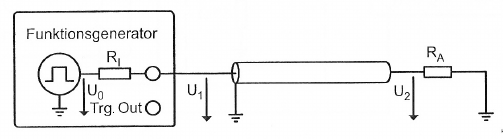
\includegraphics[width=.8\textwidth]{abb-1-5.png}
\end{figure}

Für die Längenabhängigkeit erhalten wir also:
\[
	R_\text{in}(l) = Z' l + R_\text A
\]

\subsection{Aufgabe D}

\begin{quote}
	Wie groß ist die Eingangsimpedanz $Z$ eines verlustfreien Kabels mit
	Wellenwiderstand $Z = \SI{50}\ohm$ und einem offenen Leitungsende für eine
	Sinusspannung der Frequenz $\omega$ und der Wellenlänge auf dem Kabel
	$\lambda$ in Abhängigkeit der Länge $l$ des Kabels ($0 < l < \lambda$)?
\end{quote}

Nach \eqref{eq:1.14} ist der Wellenwiderstand:
\begin{equation}
	\label{eq:D1}
	Z := \frac{U_\text h(x)}{I_\text h(x)}
\end{equation}

Wäre nicht die rücklaufende Welle, wäre hier einfach $Z_\text{in} = Z$. In dieser Aufgabe habe ich zwar schon $Z$, allerdings reicht das nicht aus. Ich brauche:
\begin{equation}
	\label{eq:D2}
	Z_\text{in}
	= \frac{U_\text h (l) + U_\text r (l)}{I_\text h (l) + I_\text r (l)}
\end{equation}

In der Anleitung steht für die offene Leitung
\[
	I_\text r(l) + I_\text h(l) = 0
\]
sowie
\[
	U_\text r(l) - U_\text h(l) = 0.
\]

Mit \eqref{eq:1.7} können wir herleiten:
\begin{align*}
	U_\text r(l) &= U_\text h(l) \\
	U_\text h(0) \eup^{-\Upsilon x} \eup^{\iup \omega t} &= U_\text r(0) \eup^{\Upsilon x}) \eup^{\iup \omega t} \\
	U_\text h(0) \eup^{-\Upsilon x} &= U_\text r(0) \eup^{\Upsilon x}) \\
	U_\text h(0) \eup^{-2 \Upsilon x} &= U_\text r(0) \\
\end{align*}

Für den Strom geht dies analog und führt auf die gleiche Phase zwischen ein-
und ausgehender Welle. Damit können wir \eqref{eq:D2} umschreiben und erhalten:
\[
	Z_\text{in}
	= \frac{U_\text h (l)}{I_\text h (l)} (1 + \eup^{-2 \Upsilon x}
\]

In diese Relation setzen wir wiederum \eqref{eq:D1} ein und vereinfachen so zu:
\[
	Z_\text{in}
	= Z (1 + \eup^{-2 \Upsilon x}
\]

Das Kabel war als verlustfrei vorgegeben, es gibt also keinen Strom zwischen Leiter und Masse. Damit ist $Y = Y' = 0$ Aus \eqref{eq:1.6} folgt damit, dass $\Upsilon = 0$ ist. Dadurch ist der Phasenfaktor in der obigen Formel einfach eins.

Wir erhalten das Ergebnis:
\[
	Z_\text{in} = 2 Z
\]

Dies ist unabhängig von der Länge und der Wellenlänge sowie der Frequenz.

%%%%%%%%%%%%%%%%%%%%%%%%%%%%%%%%%%%%%%%%%%%%%%%%%%%%%%%%%%%%%%%%%%%%%%%%%%%%%%%
%                      Versuchsaufbau und -durchführung                      %
%%%%%%%%%%%%%%%%%%%%%%%%%%%%%%%%%%%%%%%%%%%%%%%%%%%%%%%%%%%%%%%%%%%%%%%%%%%%%%%

\section{Versuchsaufbau und -durchführung}

\subsection{Seriennummern}

Die Seriennummern unserer Geräte haben wir in Tabelle \ref{tb:seriennummern}
aufgelistet.

\begin{table}[hb]
	\center
	\caption{Seriennummern unserer Geräte}
	\label{tb:seriennummern}
	\begin{tabular}{ll}
		Gerät & Seriennummer \\
		\hline
		Oszillograph & \\
		Funktionsgenerator & \\
		Kabel HH 2500 & \\
		Kabelkasten (RG-58 C/U) & \\
		Differenzierglied & \\
		Differenzierglied mit \SI{2.2}{\kilo\ohm} Anpassung & \\
		Anpasswiderstand: \SI{2.45}{\kilo\ohm} & \\
		Abschlusswiderstand: \SI{2.5}{\kilo\ohm} und \SI{50}{\ohm} & \\
		Einstellbarer Abschlusswiderstand: \SIrange{0}{10}{\kilo\ohm} &
	\end{tabular}
\end{table}

\subsection{Versuchsaufgabe 1: Differenzierglied}

\subsection{Versuchsaufgabe 2: Impulse auf Kabeln}

\subsection{Versuchsaufgabe 3: Leitungsabschluss, Verzögerungszeit}

\subsection{Versuchsaufgabe 4: Klippkabel, Dämpfung}

\subsection{Versuchsaufgabe 5: \SI{50}{\ohm} Kabel RG-58 C/U}

\subsubsection{Teil a}

\begin{quote}
	Warum macht sich eine kleine Bandbreite besonders bei der Übertragung von
	Rechtecksignalen bemerkbar?
\end{quote}

Entwickelt man ein Rechtecksignal in eine Fourierreihe, so fallen die
Amplituden der hohen Frequenzen nur langsam ab, weil die Funktion nicht
besonders glatt ist. Dies bedeutet, dass sehr viele hohe Frequenzen mit
einbezogen werden müssen, damit die Summe wie ein Rechteck aussieht. Bei einer
kleinen Bandbreite ist allerdings genau dies das Problem: Hohe Frequenzen
werden abgeschnitten, da sie besonders gedämpft werden. So wird das Rechteck an
den Ecken etwas abgerundet.

%%%%%%%%%%%%%%%%%%%%%%%%%%%%%%%%%%%%%%%%%%%%%%%%%%%%%%%%%%%%%%%%%%%%%%%%%%%%%%%
%                                 Auswertung                                  %
%%%%%%%%%%%%%%%%%%%%%%%%%%%%%%%%%%%%%%%%%%%%%%%%%%%%%%%%%%%%%%%%%%%%%%%%%%%%%%%

\section{Auswertung}

%%%%%%%%%%%%%%%%%%%%%%%%%%%%%%%%%%%%%%%%%%%%%%%%%%%%%%%%%%%%%%%%%%%%%%%%%%%%%%%
%                                  Ergebnis                                   %
%%%%%%%%%%%%%%%%%%%%%%%%%%%%%%%%%%%%%%%%%%%%%%%%%%%%%%%%%%%%%%%%%%%%%%%%%%%%%%%

\section{Ergebnis}

\IfFileExists{\bibliographyfile}{
	\bibliography{\bibliographyfile}
}{}

\end{document}

% vim: spell spelllang=de
